\documentclass[a4paper]{article}

%%% usepackage %%%
\usepackage[right=2cm, left=2cm, bottom=2cm, top=2cm]{geometry}
\usepackage{listings}
\usepackage{fancyvrb}
\usepackage{graphicx}
\usepackage{color}
\usepackage{float}
\usepackage{xepersian}
\settextfont{Dubai}
\fontsize{30}{12}\selectfont


%%% newcommand %%%
\newcommand{\mycodeinput}[1]{\noindent \lstinputlisting[firstline=0, lastline=200, caption=#1, captionpos=b]{#1}}
\newcommand{\emailone}{\texttt{abbas.yazdanmehr1@gmail.com}}
\newcommand{\fulltitle}[2]{\title{#1 \\ #2}}
\newcommand{\myinf}{
	\author{
عباس یزدان مهر
\\
99243077\\
\and
پدرام رمضان زاده\\
99243085
	}
}
\newcommand{\goodbye}{\begin{center}{\huge
پایان
}\end{center}}


\definecolor{dkgreen}{rgb}{0,0.6,0}
\definecolor{gray}{rgb}{0.5,0.5,0.5}
\definecolor{mauve}{rgb}{0.58,0,0.82}

\lstset{frame=tb,
  language=VHDL,
  aboveskip=3mm,
  belowskip=3mm,
  showstringspaces=false,
  columns=flexible,
  basicstyle={\small\ttfamily},
  numbers=none,
  numberstyle=\tiny\color{gray},
  keywordstyle=\color{blue},
  commentstyle=\color{dkgreen},
  stringstyle=\color{mauve},
  breaklines=true,
  breakatwhitespace=true,
  tabsize=3
}


\begin{document}

\fulltitle{
طراحی سیستم های دیجیتال
}{
پروژه نهایی \\
مهندسی کامپیوتر, دانشگاه شهید بهشتی
}

\myinf

\maketitle

\newpage

\section{ماشین حساب}

\subsection{ماشین حالات}
\begin{figure}[H]
	\begin{small}
		\begin{center}
			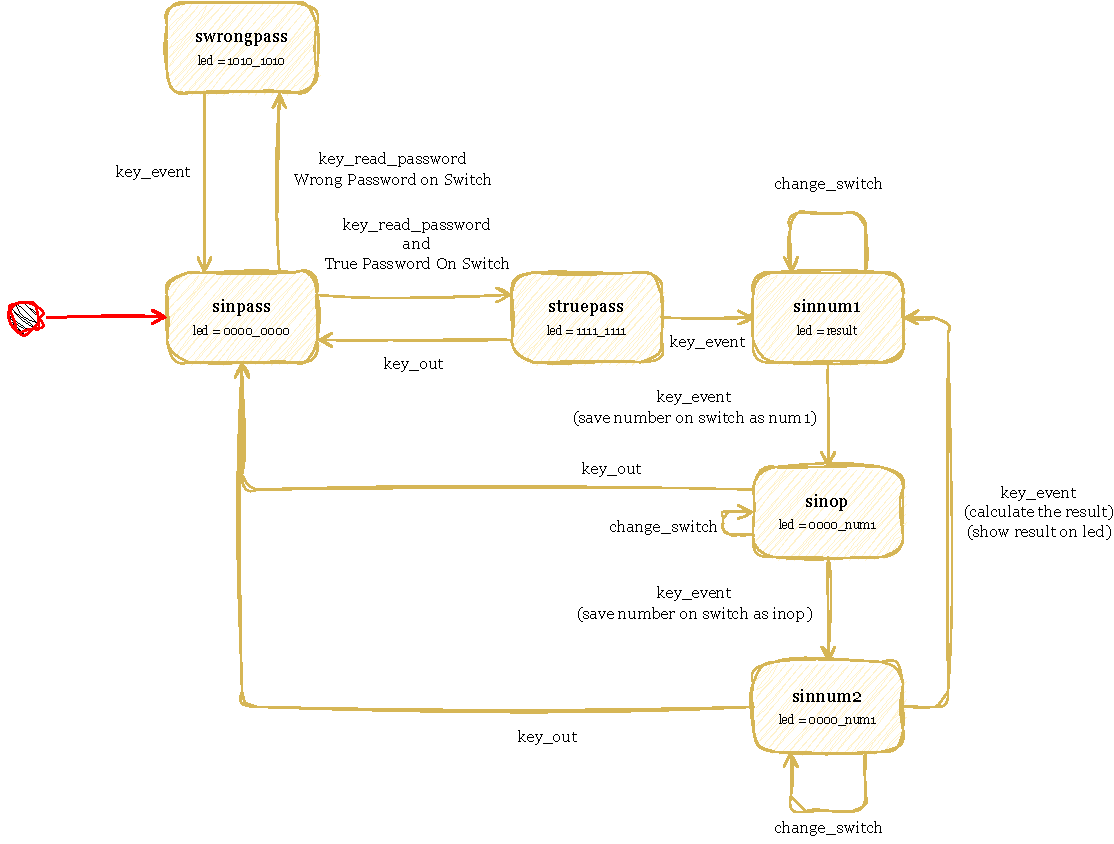
\includegraphics[width=0.95\textwidth]{figures/fsm.pdf}
		\end{center}
		\caption{ماشین حالات}
		\label{fig:fsm}
	\end{small}
\end{figure}


\subsection{کد}
\begin{latin}
    \mycodeinput{code/calcul.vhd}
\end{latin}

\subsection{شبیه سازی}
\subsubsection{کد تست}

\begin{latin}
  \mycodeinput{code/calcultb.vhd}
\end{latin}

\subsubsection{خروجی تست}
\begin{figure}[H]
	\begin{small}
		\begin{center}
			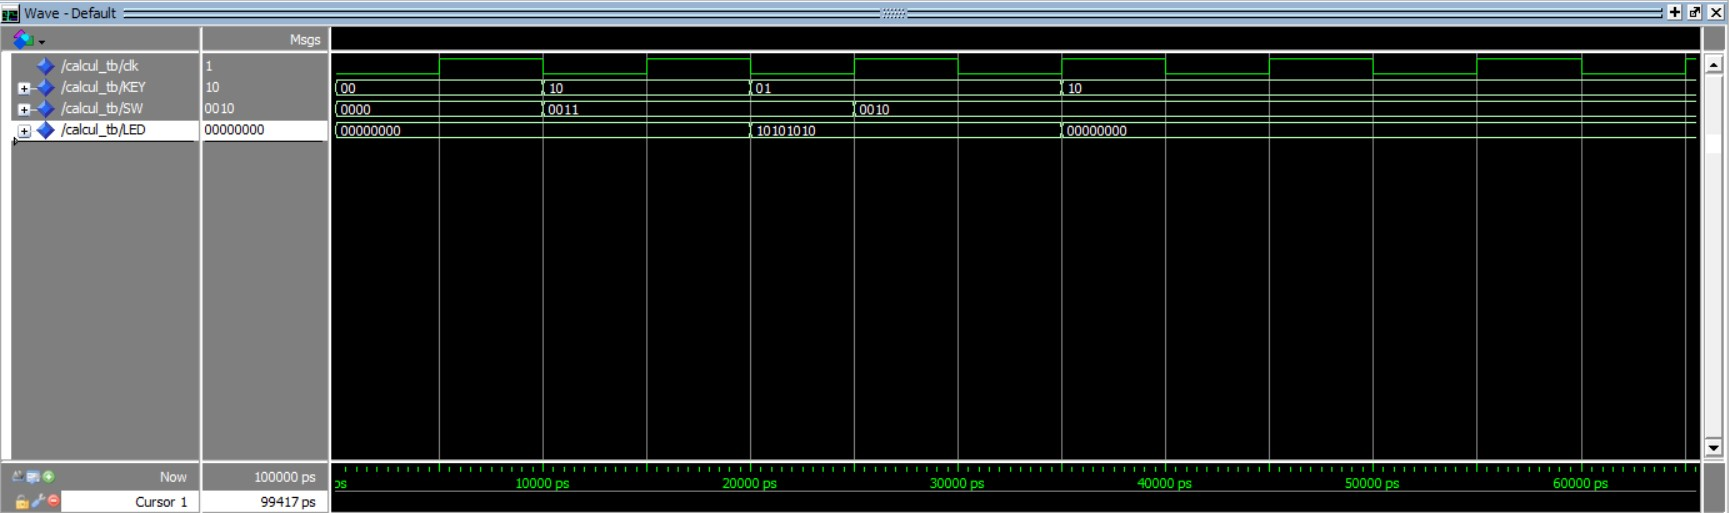
\includegraphics[width=0.95\textwidth]{figures/sim1.jpg}
		\end{center}
		\caption{شبیه سازی - واردکردن رمز نادرست}
		\label{fig:sim1}
	\end{small}
\end{figure}

\begin{figure}[H]
	\begin{small}
		\begin{center}
			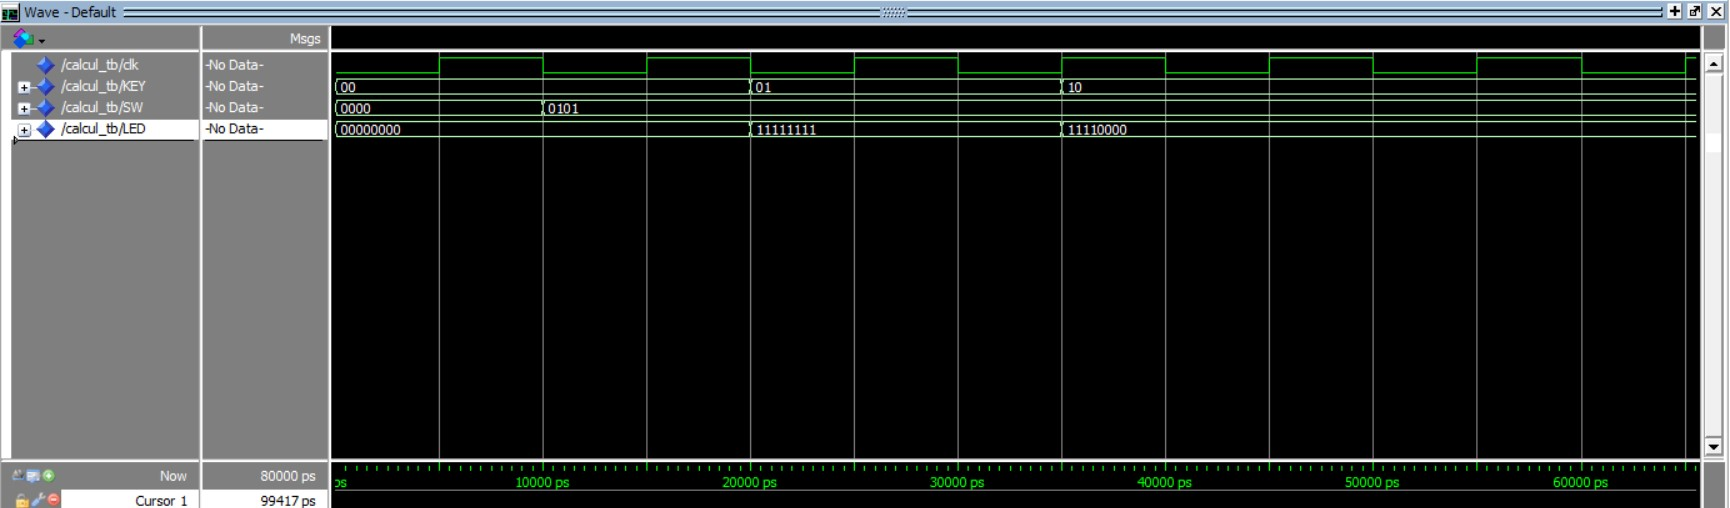
\includegraphics[width=0.95\textwidth]{figures/sim2.jpg}
		\end{center}
		\caption{شبیه سازی - واردکردن رمز درست}
		\label{fig:sim2}
	\end{small}
\end{figure}

\begin{figure}[H]
	\begin{small}
		\begin{center}
			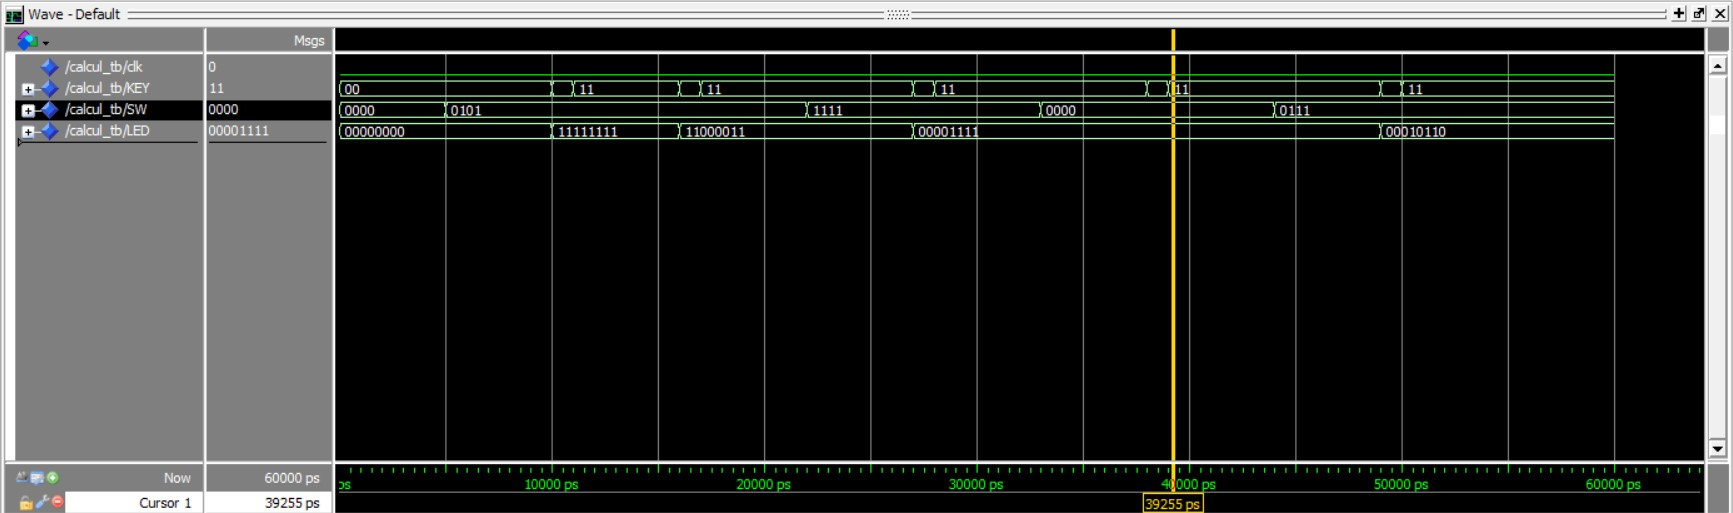
\includegraphics[width=0.95\textwidth]{figures/sim3.jpg}
		\end{center}
		\caption{شبیه سازی - یک روند از انجام کامل عملیات}
		\label{fig:sim3}
	\end{small}
\end{figure}

\newpage
\goodbye
\end{document}
